%===============================================================================
% ADT Developer Guide
%===============================================================================
% $Id: developer-guide.tex 248 2005-01-30 23:25:27Z thom $
%===============================================================================


%===============================================================================
% Configuration
%===============================================================================


%-------------------------------------------------------------------------------
% \documentclass and \usepackage directives
%-------------------------------------------------------------------------------
\documentclass[a4paper,fleqn,titlepage]{article}
%\usepackage{ngerman}
\usepackage[latin1]{inputenc}
\usepackage[T1]{fontenc}
\usepackage[small,hang,bf]{caption2}
\usepackage{fancyhdr}
\usepackage[nice]{nicefrac}
\usepackage{color,listings}
\usepackage{alltt}


% Compilation with latex or pdflatex?
\newif\ifpdf 
\ifx\pdfoutput\undefined 
  \pdffalse
\else
  \pdfoutput=1 
  \pdftrue 
\fi 

% Compilation with pdflatex
\ifpdf
 
  \usepackage[pdftex]{graphicx}

  \usepackage[
    pdftex,
    a4paper,
    bookmarks,
    pdfstartview=FitH,    % starts with page width
    bookmarksopen,        % opens index
    bookmarksnumbered,    % index with numbering
    colorlinks,           % links with color, otherwise with border
    linkcolor=blue,       % Standard red
    citecolor=blue,       % Standard green
    urlcolor=magenta,     % Standard cyan
    filecolor=blue
  ]{hyperref} 

  \pdfinfo{
    /Title      (EiffelRSS ADT Developer Guide)
    /Author     (Thomas Weibel, Martin Luder, Michael K�ser)
    /Subject    (Eiffel programming)
    /Keywords   (Programming, EiffelRSS)
  }

  % Use default Acrobat reader fonts
  \usepackage{mathpazo}

  % Use CM fonts (increases document size)
  % \usepackage{ae}

% Compilation with latex
\else 

  \usepackage{graphicx} 

\fi


%-------------------------------------------------------------------------------
% Configure \maketitle
%-------------------------------------------------------------------------------
\title{EiffelRSS \\ ADT \\ Developer Guide}
\author{
  Michael K\"aser <kaeserm@student.ethz.ch>
  \and 
  Martin Luder <luderm@student.ethz.ch>
  \and 
  Thomas Weibel <weibelt@student.ethz.ch>
}
\date{\today}


%-------------------------------------------------------------------------------
% Configure fancyhdr
%-------------------------------------------------------------------------------
\pagestyle{fancy}

\renewcommand{\headrulewidth}{0.1 pt}
\renewcommand{\footrulewidth}{0.1 pt}

\fancypagestyle{plain}{
  \lhead{\nouppercase{\leftmark}}
  \chead{}
  \rhead{\thepage}
  \lfoot{EiffelRSS}
  \cfoot{}
  \rfoot{ADT Developer Guide}
}

\lhead{\nouppercase{\leftmark}}
\chead{}
\rhead{\thepage}

\lfoot{EiffelRSS}
\cfoot{}
\rfoot{ADT Developer Guide}


%-------------------------------------------------------------------------------
% Configure listings
%-------------------------------------------------------------------------------
\lstset{showstringspaces=false,
  breaklines=true,
  breakindent=0pt,
  prebreak=\mbox{\tiny$\searrow$},
  postbreak=\mbox{{\color{blue}\tiny$\rightarrow$}},
  frame=trBL,
  framerule=0.75pt,
  framesep=4pt,
  rulesep=0.75pt  
}


%-------------------------------------------------------------------------------
% Common configuration
%-------------------------------------------------------------------------------
\setlength{\parindent}{0em}
\setlength{\parskip}{1.5ex plus0.5ex minus0.5ex}
\sloppy
\setlength{\mathindent}{0em}


%-------------------------------------------------------------------------------
% Commandos
%-------------------------------------------------------------------------------
\newcommand{\hr}{\rule{\textwidth}{1pt}}


%===============================================================================
% Document
%===============================================================================
\begin{document}

\begin{titlepage}
  \newlength{\centeroffset}
  \setlength{\centeroffset}{-0.5\oddsidemargin}
  \addtolength{\centeroffset}{0.5\evensidemargin}

  \thispagestyle{empty}

  \noindent
\includegraphics[width=\textwidth]{../../figures/big_ETH}\\[-3mm]
  \hr

  \vspace*{\stretch{1}}

  \makebox[0pt][l]{
    \begin{minipage}{\textwidth}
      \flushright{
        \Huge\bfseries EiffelRSS
      }

      \noindent\rule{\textwidth}{3pt}\\[2.5ex]

      \hfill\emph{
        \Large ADT Developer Guide
      }
    \end{minipage}
  }

  \vspace{\stretch{1}}

  \makebox[0pt][l]{
    \begin{minipage}{\textwidth}
      \flushright{
        \bfseries 
        Michael K\"aser <kaeserm@student.ethz.ch>\\[0.3ex]
        Martin Luder <luderm@student.ethz.ch>\\[0.3ex]
        Thomas Weibel <weibelt@student.ethz.ch>\\[0.3ex]
      }
    \end{minipage}
  }

  \vspace{\stretch{1}}

  \noindent\hr\\[1mm]
  
\includegraphics[width=\textwidth]{../../figures/big_inf}
\end{titlepage}

% Use roman page numbering
\pagenumbering{roman}

\begin{abstract}
  \texttt{ADT} contains the deferred classes \texttt{SORTABLE} and
  \texttt{ORDER\_RELATION} which can be used to implement sortable
  structures.
\end{abstract}

\clearpage
\tableofcontents

\clearpage
\listoffigures

\newpage

\section{Overview}
\label{sec:overview}

% Set page counter to zero
\setcounter{page}{0} 

% Use arabic page numbering
\pagenumbering{arabic}

\textit{ADT} is a three letter acronym for \textit{abstract data type}.

\texttt{ADT} contains the deferred classes \texttt{SORTABLE} and
\texttt{ORDER\_RELATION} which can be used to implement sortable
structures. 

\texttt{SORTABLE\_TWO\_WAY\_LIST} inherits from \texttt{SORTABLE} and
\texttt{TWO\_WAY\_LINKED\_LIST} to implement a sortable doubly-linked
list.

See figure \ref{fig:cluster} for an overview of the cluster.

\begin{figure}[htbp]
  \centering
  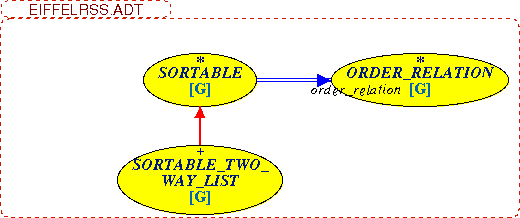
\includegraphics[scale=.6]{./figures/EIFFELRSS_ADT}
  \caption{BON diagram of cluster \texttt{ADT}}
  \label{fig:cluster}
\end{figure}

Figure \ref{fig:classes} shows the class \texttt{SORTABLE\_TWO\_WAY\_LIST}.

\begin{figure}[htbp]
  \centering
  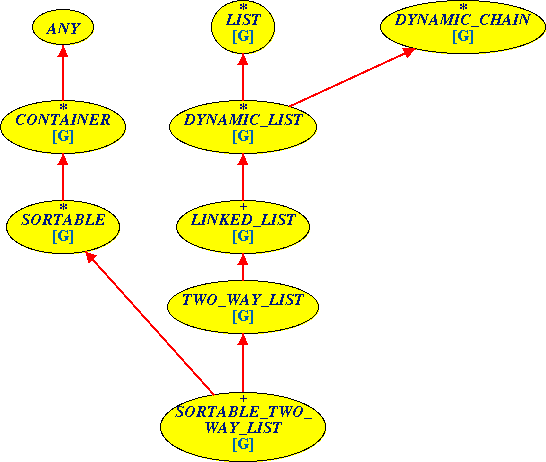
\includegraphics[scale=.5]{./figures/SORTABLE_TWO_WAY_LIST}
  \caption{BON diagram of class \texttt{SORTABLE\_TWO\_WAY\_LIST}}
  \label{fig:classes}
\end{figure}

\newpage

\section{Usage}
\label{sec:usage}

The following example shows a simple use-case for
\texttt{SORTABLE\_TWO\_WAY\_LIST}.

\subsection{SORT\_BY\_NAME - a sorter for an address class}

\begin{lstlisting}[language=Eiffel]
class
  SORT_BY_NAME[G -> ADDRESS]
  
inherit
  ORDER_RELATION[G]

feature -- Criterion

  ordered (first, second: G): BOOLEAN is
      -- Are `first' and `second' ordered (true if `first' < `second')
    require else
      first_non_void: first /= Void
      second_non_void: second /= Void
    do
      Result := first.name < second.name
    end

end -- class SORT_BY_NAME
\end{lstlisting}

\subsection{ADDRESS - a simple address class}

\begin{lstlisting}[language=Eiffel]
class
  ADDRESS
  
inherit
  ANY
    redefine
      out
    end
  
create
  make
  
feature -- Initialization

  make (a_name: STRING; a_planet: STRING; a_phone_number: INTEGER) is
      -- Create a new address with name, street, city and phone number
    require
      non_empty_name: a_name /= Void and then not a_name.is_empty
      non_empty_planet: a_planet /= Void and then not a_planet.is_empty
    do
      name := a_name
      planet := a_planet
      phone_number := a_phone_number
    ensure
      name_set: name = a_name 
      planet_set: planet = a_planet
      phone_number_set: phone_number = a_phone_number
    end
    
feature -- Arguments

  name, planet: STRING
  
  phone_number: INTEGER
    
feature -- Output

  out: STRING is
      -- Returns a string representation of an address object
    do
      Result := "- Name: " + name + "%N- Planet: " + planet + "%N- Phone number: " + phone_number.out + "%N"
    end

end -- class ADDRESS
\end{lstlisting}


\subsection{Using ADDRESS and SORT\_BY\_NAME}

\begin{lstlisting}[language=Eiffel]
class
  ADDRESS_BOOK

create
  make

feature -- Initialization

  make is
      -- Creation procedure.
    do
      create address_list.make
      
      create address.make ("Zaphod", "Betelgeuse", 12)
      address_list.extend (address)
      
      create address.make ("Marvin", "Sirius", 96)
      address_list.extend (address)
      
      create address.make ("Ford", "Betelgeuse", 25)
      address_list.extend (address)
      
      create address.make ("Trillian", "Earth", 23)
      address_list.extend (address)
      
      create address.make ("Arthur", "Earth", 42)
      address_list.extend (address)
      
      create address.make ("Slartibartfast", "Magrathea", 43)
      address_list.extend (address)
      
      io.put_string ("No particular sorting:%N")
      io.put_string ("======================%N")
      address_list.do_all (agent print_address)
      
      io.put_string ("By name:%N")
      io.put_string ("========%N")
      address_list.set_order (create {SORT_BY_NAME[ADDRESS]})
      address_list.sort
      address_list.do_all (agent print_address)
    end
    
feature -- Arguments

  address_list: SORTABLE_TWO_WAY_LIST[ADDRESS]
  address: ADDRESS

feature -- Output

  print_address (an_address: ADDRESS) is
      -- Prints address
    require
      address_non_void: address /= Void
    do
      io.put_string (an_address.out + "%N")
    end

end -- class ADDRESS_BOOK
\end{lstlisting}


\section{Features of SORTABLE\_TWO\_WAY\_LIST}
\label{sec:features}

Because \texttt{SORTABLE\_TWO\_WAY\_LIST} inherits from
\texttt{TWO\_WAY\_LIST}, all features of this class can also be
applied to a \texttt{SORTABLE\_TWO\_WAY\_LIST} object, e.g.  \texttt{extend},
\texttt{prune} etc.


\subsection{Initialization}
\label{sec:initialization}


\subsubsection{make}

\begin{lstlisting}[language=Eiffel]
make is
  -- Create an empty two way list, with no order relation
\end{lstlisting}


\subsubsection{make\_with\_order\_relation }

\begin{lstlisting}[language=Eiffel]
make_with_order_relation (an_order_relation: ORDER_RELATION[G]) is
  -- Create an empty two way list, with `an_order_relation' as order relation
\end{lstlisting}


\subsection{Access}
\label{sec:access}


\subsubsection{has}

\begin{lstlisting}[language=Eiffel]
has (v: G): BOOLEAN is
  -- Does structure include `v'?
  -- (Reference or object equality,
  -- based on `object_comparison'.)
\end{lstlisting}


\subsection{Order relation}
\label{sec:order-relation}


\subsubsection{has\_order}

\begin{lstlisting}[language=Eiffel]
has_order: BOOLEAN is
  -- Is an order relation defined?
\end{lstlisting}


\subsubsection{set\_order}

\begin{lstlisting}[language=Eiffel]
set_order (an_order_relation: ORDER_RELATION[G]) is
  -- Set the order relation.
\end{lstlisting}


\subsection{Sorting}
\label{sec:sorting}


\subsubsection{sort}

\begin{lstlisting}[language=Eiffel]
sort is
  -- Sort all items.
\end{lstlisting}


\subsubsection{sorted}

\begin{lstlisting}[language=Eiffel]
sorted: BOOLEAN is
  -- Is the structure sorted?
\end{lstlisting}

\end{document}
